\documentclass{article}
\usepackage{../../Self_Style}

\title{Phys 20AL Week 8 Lab Report: Path of Light}
\author{Zih-Yu Hsieh}
\date{\today}

\begin{document}
\maketitle

\tableofcontents

\section{Introduction}
For the light's traveling path, intuition and some quite limited daytime observation would conclude that light travels in a straight path. However, extending suchh observation to the scenarios where light travels in different medium (for instance, water and air), it can be observed that the light now travels not in a straight line, but rather a bend path with change in direction happening at the surafce where the medium changes. More interesting examples can be seen in mirage - when light travels through air with different temperature layers, not only the path bent, but in fact curved in a way so that objects can be observed at a location where it's not supposed to be seen (for instance, cloud on the ground, and ships in the air).

Here, the simplest model to describe such change of path is through index of refraction - the ratio of speed of light (in vacuum) over the speed of light (in the medium). And, given the two mediums with index of refraction $n_,n_2$, as the light travels from medium 1 to 2, with incident angle away from the normal being $\theta_1,\theta_2$, then Snell's Law states the relation $n_1\sin(\theta_1)=n_2\sin(\theta_2)$.

The aim for the experiment is to study the path that light travels: First it'll be focused on using Snell's Law to calculate a half-cylinder's index of refraction (that's independent of the frequency of the light). Later on it'll be focused on using the prism to get a frequency-dependent index of refraction for a prism instead (or testing the dispersion of light).

\newpage

\section{Experimental Setup}
The equipments include: A light source (with both white light, and RGB lights), a protractor, and transparent half-cylinder and triangular prism.

The equipment setup is also simple: setup the light so the path of the light passes through where the half-cylinder and the triangular prism are going to be at, and put a protractor below for angle measurement.
\begin{figure}[h!]
    \centering
    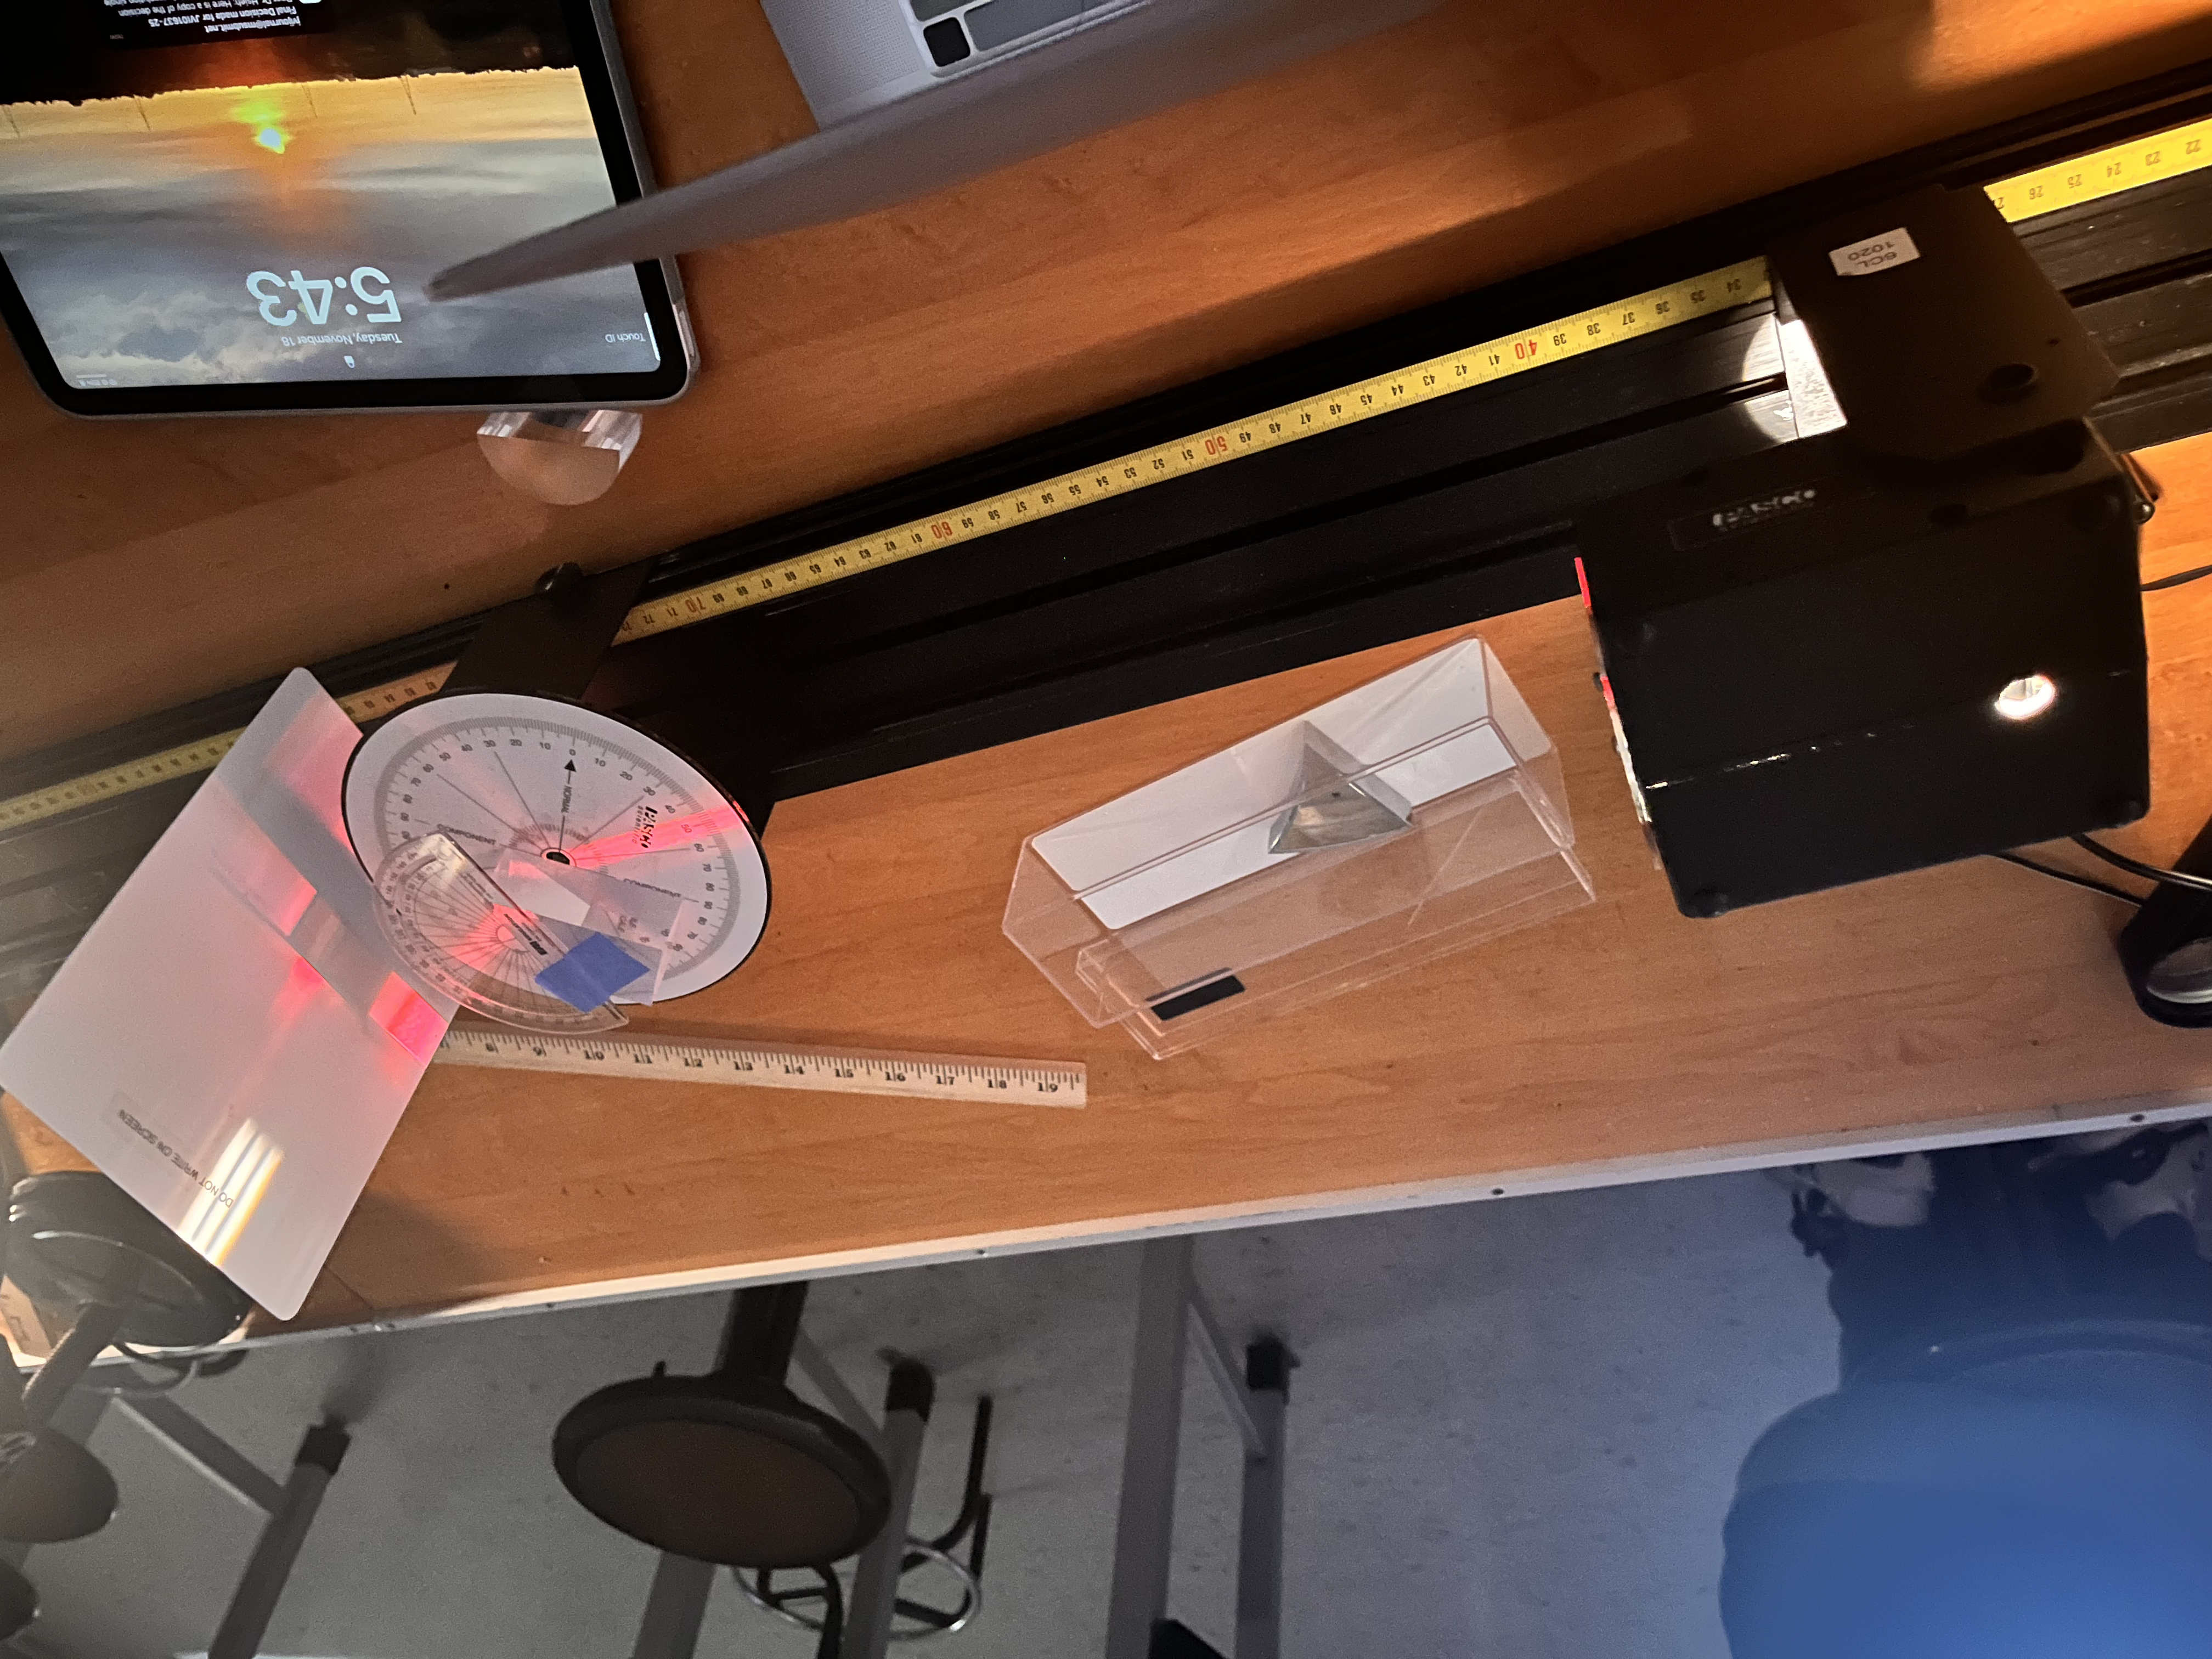
\includegraphics[width=100mm]{lat_setup8.png}
    \caption{The actual lab setup picture}
\end{figure}

\section{Quantity to Measure, and Method of Measure}
For measuring the index of refraction through Snell's Law, the incident angle of the light away from the normal line of the surface well be measured (for both the input and output light), and it'll be measured through the protractor.

For both experiments (using the white light and the RGB light), there are total of $5$ incident angles: $10,20,30,40,50^\circ$ that are used as manipulated variable. For the second experiment specifically (when testing the frequency dependence of index of refraction, using the RGB light), the color (or frequency) of the light is also a manipulated variable.

For each pair of manipulated variables, total of 3 trials fo measurement will be performed.

\hfil

\section{Experimental Procedure}
\subsection{Frequency Independent Experiment}
It'll follow the procedure below:
\begin{enumerate}
    \item Turn on the white light, and put the half-cylinder on the path of the light, with the flat side facing toward the light.
    \item Tweak the cylinder, so the light is passing directly through the center of the half-cylinder (or, the center point of the semicircle).
    \item Adjust the angle of the cylinder, so the light has incident angle as one of the angles to be measured. Then, measure the incident angle of the output light.
    \item Repeat Step 3 for all the other angles await to be measured.
    \item Repeat Step 3-4 for a total of 3 trials to get all the desired measurements.
\end{enumerate}
Afterward, using the gathered data to calculate the index of refraction of the half-cylinder, use it to predict the critical angle, and test how well the prediction is experimentally.

\subsection{Frequency Dependent Experiment}
In this case, the experimental procedure is quite similar to \textbf{Subsection 4.1}, except now there are 3 different light sources - red, green, and blue. So, the experiment described above needs to be repeated for all types of light source, to get the index of refraction with respect to each frequency of light.

\hfil

\section{Experimental Data and Data Analysis}
\subsection{Frequency Independent Experiment}
Here are the experimental data:
\begin{table}[h!]
\centering
\begin{tabular}{c||c c c|c c}
\hline
\textbf{Input Angle ($ ^\circ$)} & \textbf{Trial 1} & \textbf{Trial 2} & \textbf{Trial 3} & \textbf{Average Output Angle ($ ^\circ$)} & \textbf{SD ($ ^\circ$)} \\
\hline
10 & 7.500 & 7.000 & 7.000 & 7.167 & 0.289 \\
20 & 14.000 & 13.500 & 13.500 & 13.667 & 0.289 \\
30 & 19.500 & 19.500 & 20.000 & 19.667 & 0.289 \\
40 & 25.500 & 25.500 & 25.500 & 25.500 & 0.000 \\
50 & 31.000 & 31.000 & 30.500 & 30.833 & 0.289 \\
\hline
\end{tabular}
\caption{Input vs. Output Angle of Light through Half-Cylinder}
\label{tab:freeq_indep_data}
\end{table}
Which, based on Snell's Law $n_1\sin(\theta_1)=n_2\sin(\theta_2)$, in the air one can assume $n_1=1$, hence $n_2=\frac{\sin(\theta_1)}{\sin(\theta_2)}$. Which, the uncertainty $\delta\theta_1 = 0.25^\circ$ (which is the limitation of the protractor), and $\delta\theta_2$ is calculated above in the SD column. Then, using Propogation of Uncertainty, since $\frac{\partial n_2}{\partial \theta_1}=\frac{\cos(\theta_1)}{\sin(\theta_2)}$, and $\frac{\partial n_2}{\partial \theta_2}=\frac{-\sin(\theta_1)\cos(\theta_2)}{\sin^2(\theta_2)}$, then the propogation of uncertainty is gien as follow:
\begin{align}
    \delta n_2 = \sqrt{\left(\frac{\partial n_2}{\partial \theta_1}\delta\theta_1\right)^2+\left(\frac{\partial n_1}{\partial \theta_2}\delta \theta_2\right)^2} = \sqrt{\left(\frac{\cos(\theta_1)}{\sin(\theta_2)}\delta\theta_1\right)^2+\left(\frac{-\sin(\theta_1)\cos(\theta_2)}{\sin^2(\theta_2)}\delta \theta_2\right)^2}
\end{align}
Which, the above data generate the following table about $n_2$ the index of refraction of the half-cylinder:
\begin{table}[h!]
\centering
\begin{tabular}{c ||c |c}
\hline
\textbf{Input Angle (deg)} & \textbf{$n_2$} & \textbf{$\delta n_2$} \\
\hline
10 &  1.392 & 1.974 \\
20 &  1.448 & 0.999 \\
30 &  1.486 & 0.658 \\
40 &  1.493 & 0.445 \\
50 &  1.495 & 0.367 \\
\hline
\end{tabular}
\caption{Input Angle vs. Index of Refraction of a Half-Cylinder}
\end{table}
\newpage
Which, they generate the following graph:
\begin{figure}[h!]
    \centering
    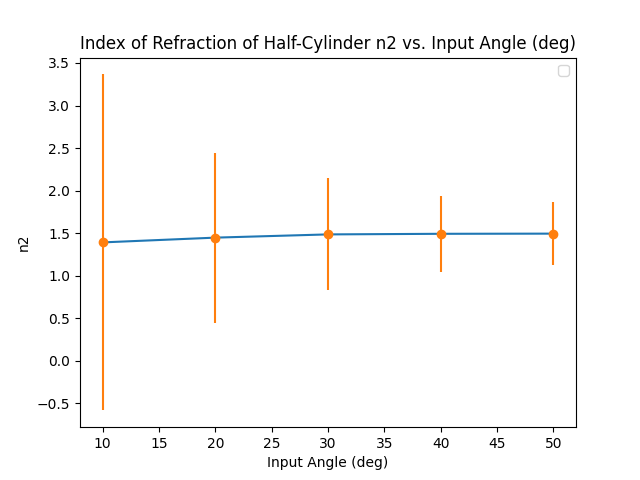
\includegraphics[width=100mm]{freq_indep.png}
    \label{fig:freq_indep_graph}
\end{figure}
Even though the eventual calculated $n_2$ values are concentrated near $1.4-1.5$, but due to the high uncertainty value $\delta n_2$, this data has a relatively low confidence of representing the actual scenario in the experiment.

Eventually, the average index of refraction $n_{2,\text{ave}} \approx 1.463$. According to this value, the critical angle $\theta_\text{crit}$ satisfies the relation $n_1\sin(\frac{\pi}{2}) = n_2\sin(\theta_\text{crit})$ (which, as the light travels from the given medium backk to the air, with input incident angle $\theta_\text{crit}$, the refracted angle is $90^\circ$, causing the total internal reflection to happen). With $n_1=\sin(\frac{\pi}{2})=1$, $\sin(\theta_\text{crit})=\frac{1}{n_2}$, or $\theta_\text{crit} = \sin\left(\frac{1}{n_{2,\text{ave}}}\right)\approx 43.136^\circ$ (the predicted critical angle). Experimentally, the following picture is taken:

\begin{figure}[h!]
    \centering
    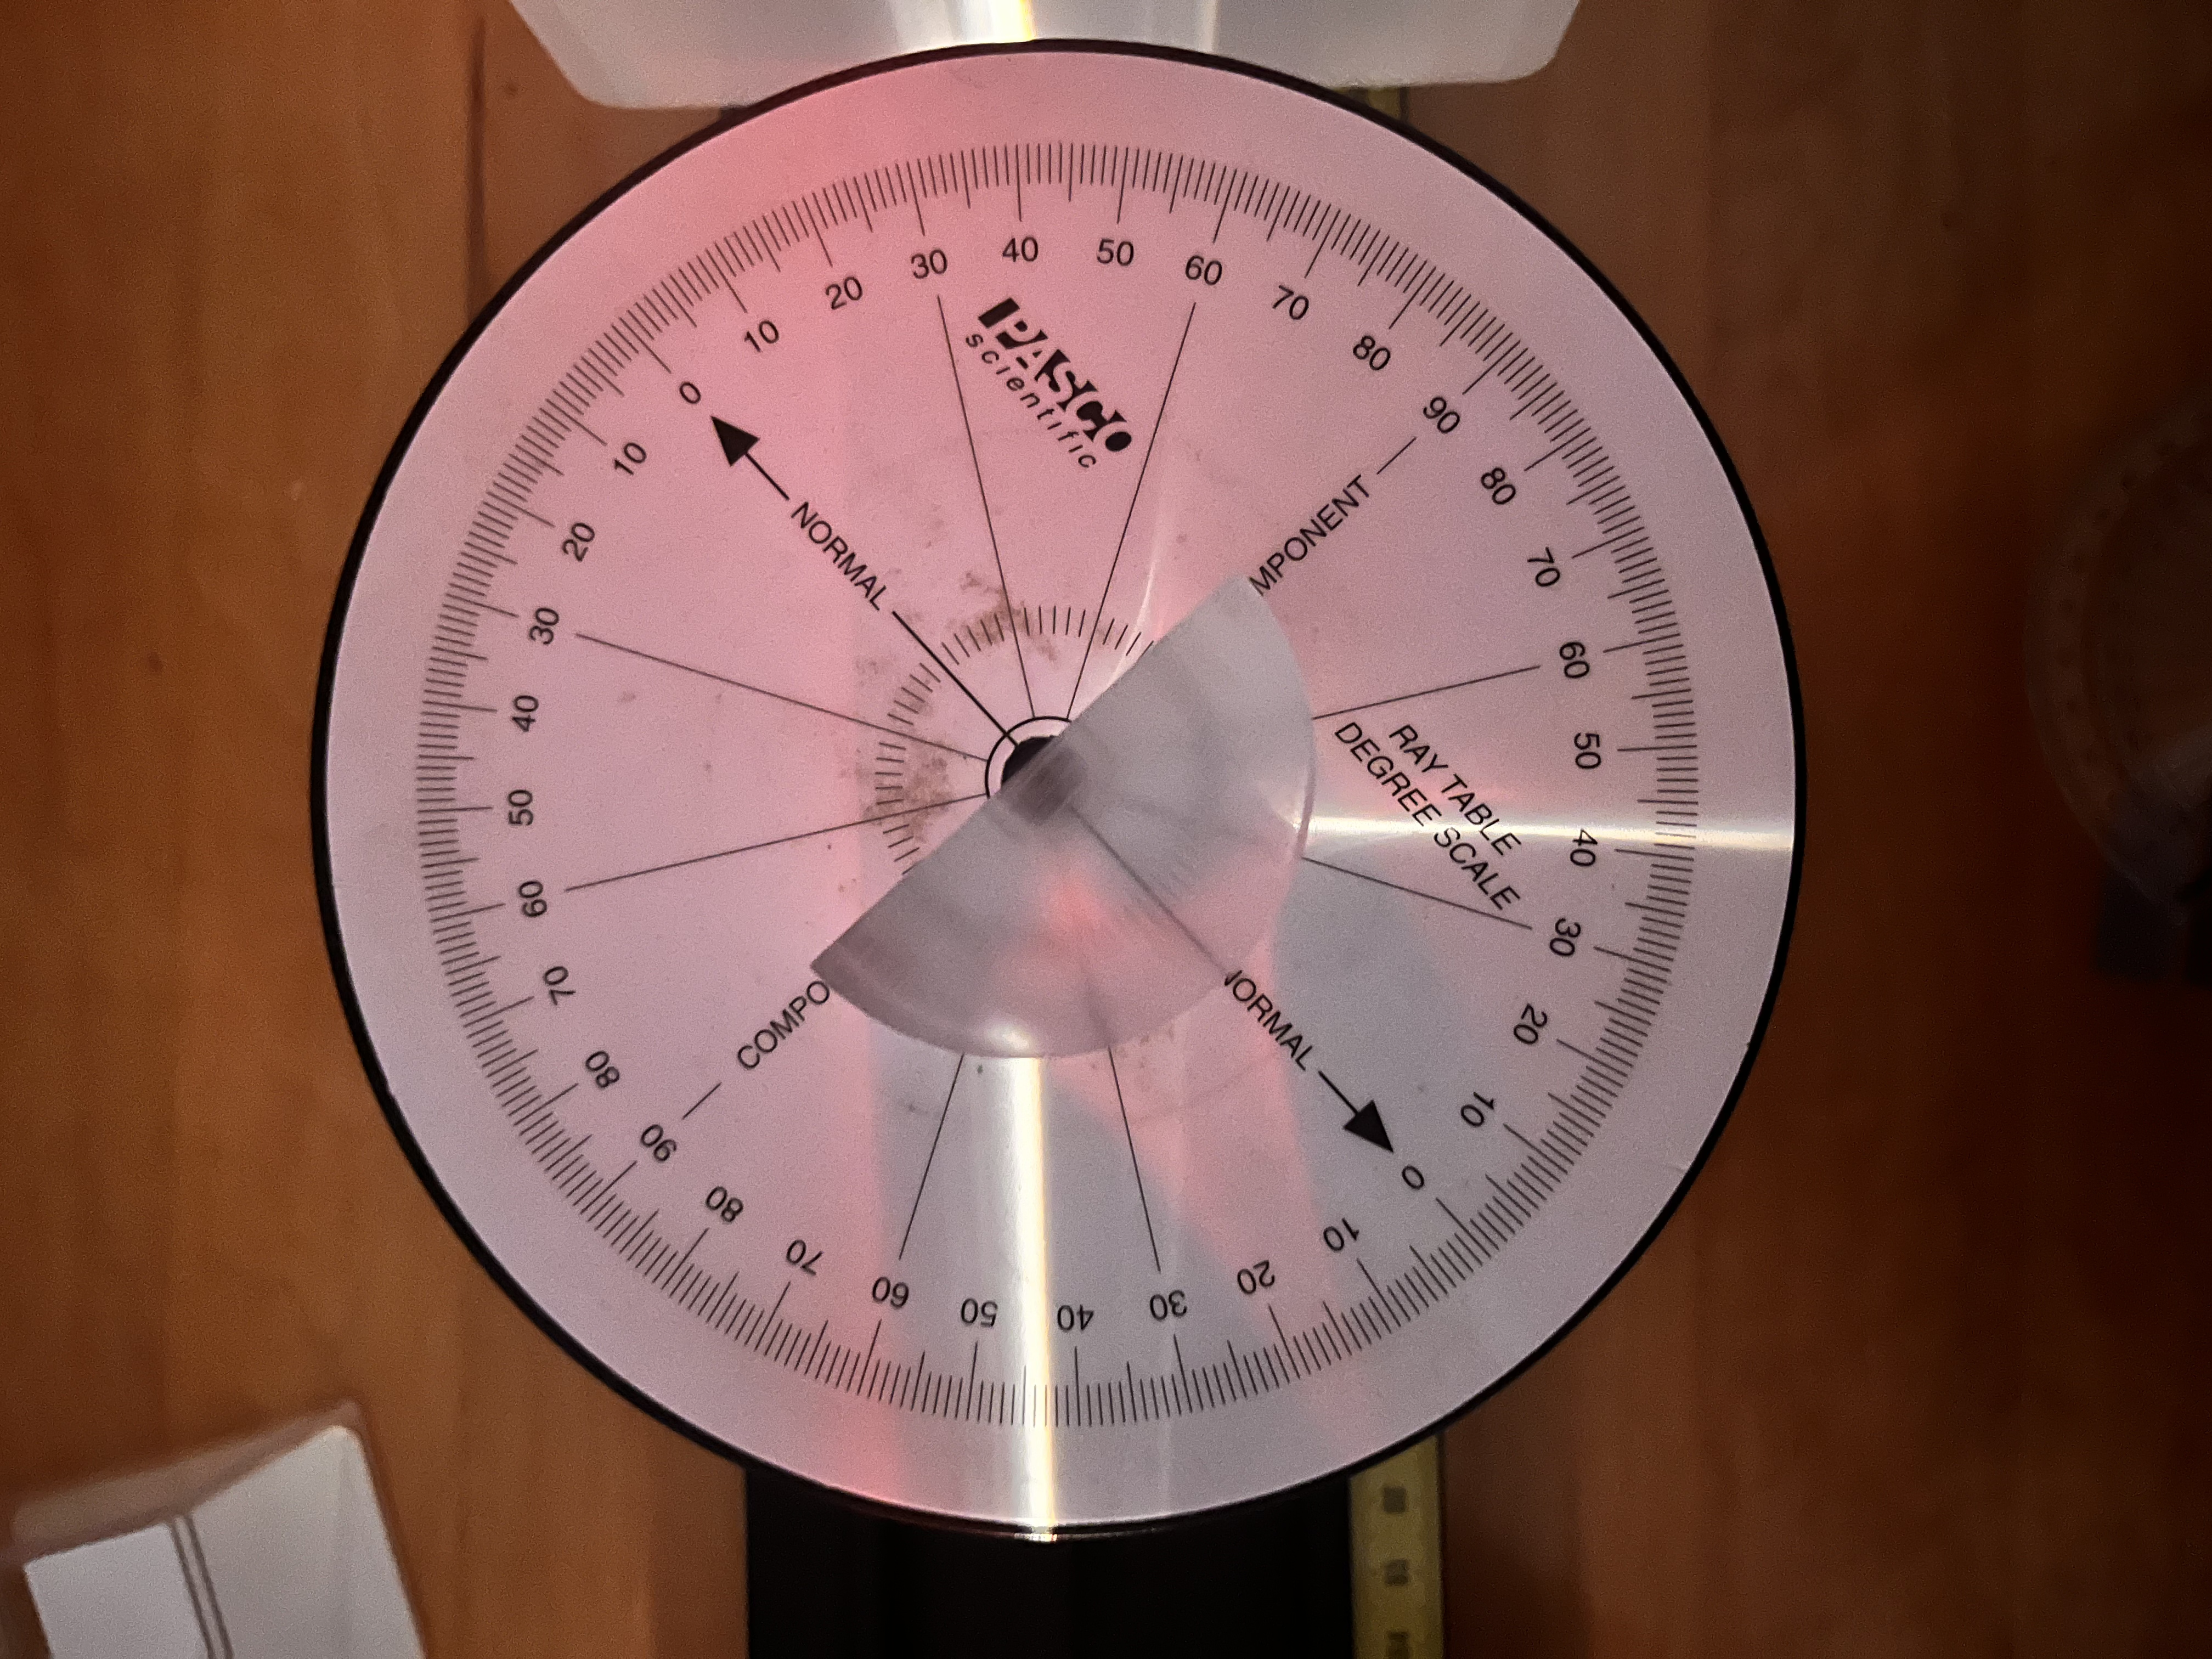
\includegraphics[width=100mm]{total_refl.png}
    \caption{Picture of Total Internal Reflection of the Half-Cylinder}
    \label{fig:total_refl}
\end{figure}

\newpage

Which, one can observe the total internal reflection starts happening when the angle is about $42^\circ$, in this case it's pretty close to the experimental prediction.

\hfil

\subsection{Frequency Dependent Experiment}
Here are the experimental data:
\begin{table}[h!]
% ------------------ Red Light ------------------
\begin{subtable}[t]{0.32\textwidth}
\centering
\begin{tabular}{c|| c c c| c c}
\hline
\textbf{Input Angle ($ ^\circ$)} & \textbf{Trial 1} & \textbf{Trial 2} & \textbf{Trial 3} & \textbf{Average Output Angle ($ ^\circ$)} & \textbf{SD}\\
\hline
10 & 22.500 & 20.000 & 19.500 & 20.667 & 1.607 \\
20 & 37.000 & 38.000 & 37.500 & 37.500 & 0.500 \\
30 & 50.000 & 49.500 & 50.000 & 49.833 & 0.289 \\
40 & 57.500 & 59.000 & 58.500 & 58.333 & 0.764 \\
50 & 68.500 & 68.500 & 69.500 & 68.833 & 0.577 \\
\hline
\end{tabular}
\caption{Red Light}
\end{subtable}

\hfill

% ------------------ Green Light ------------------
\begin{subtable}[t]{0.32\textwidth}
\centering
\begin{tabular}{c|| c c c| c c}
\hline
\textbf{Input Angle ($ ^\circ$)} & \textbf{Trial 1} & \textbf{Trial 2} & \textbf{Trial 3} & \textbf{Average Output Angle ($ ^\circ$)} & \textbf{SD}\\
\hline
10 & 27.000 & 26.000 & 26.000 & 26.333 & 0.577 \\
20 & 40.000 & 41.500 & 42.000 & 41.167 & 1.041 \\
30 & 51.500 & 51.500 & 53.000 & 52.000 & 0.866 \\
40 & 63.000 & 62.500 & 63.500 & 63.000 & 0.500 \\
50 & 71.500 & 70.000 & 70.500 & 70.667 & 0.764 \\
\hline
\end{tabular}
\caption{Green Light}
\end{subtable}

\hfill

% ------------------ Blue Light ------------------
\begin{subtable}[t]{0.32\textwidth}
\centering
\begin{tabular}{c|| c c c| c c}
\hline
\textbf{Input Angle ($ ^\circ$)} & \textbf{Trial 1} & \textbf{Trial 2} & \textbf{Trial 3} & \textbf{Average Output Angle ($ ^\circ$)} & \textbf{SD} \\
\hline
10 & 27.000 & 26.000 & 25.000 & 26.000 & 1.000 \\
20 & 41.000 & 40.000 & 41.000 & 40.667 & 0.577 \\
30 & 53.000 & 52.500 & 51.500 & 52.333 & 0.764 \\
40 & 65.000 & 63.000 & 63.500 & 63.833 & 1.041 \\
50 & 72.000 & 71.000 & 71.500 & 71.500 & 0.500 \\
\hline
\end{tabular}
\caption{Blue Light}
\end{subtable}

\caption{Input Angle vs.\ Output Angle Measurements for Red, Green, and Blue Light}
\end{table}

\newpage

Which, Based on the geometry of the triangular prism, it generates the following graph and relations:
\begin{figure}[h!]
    \centering
    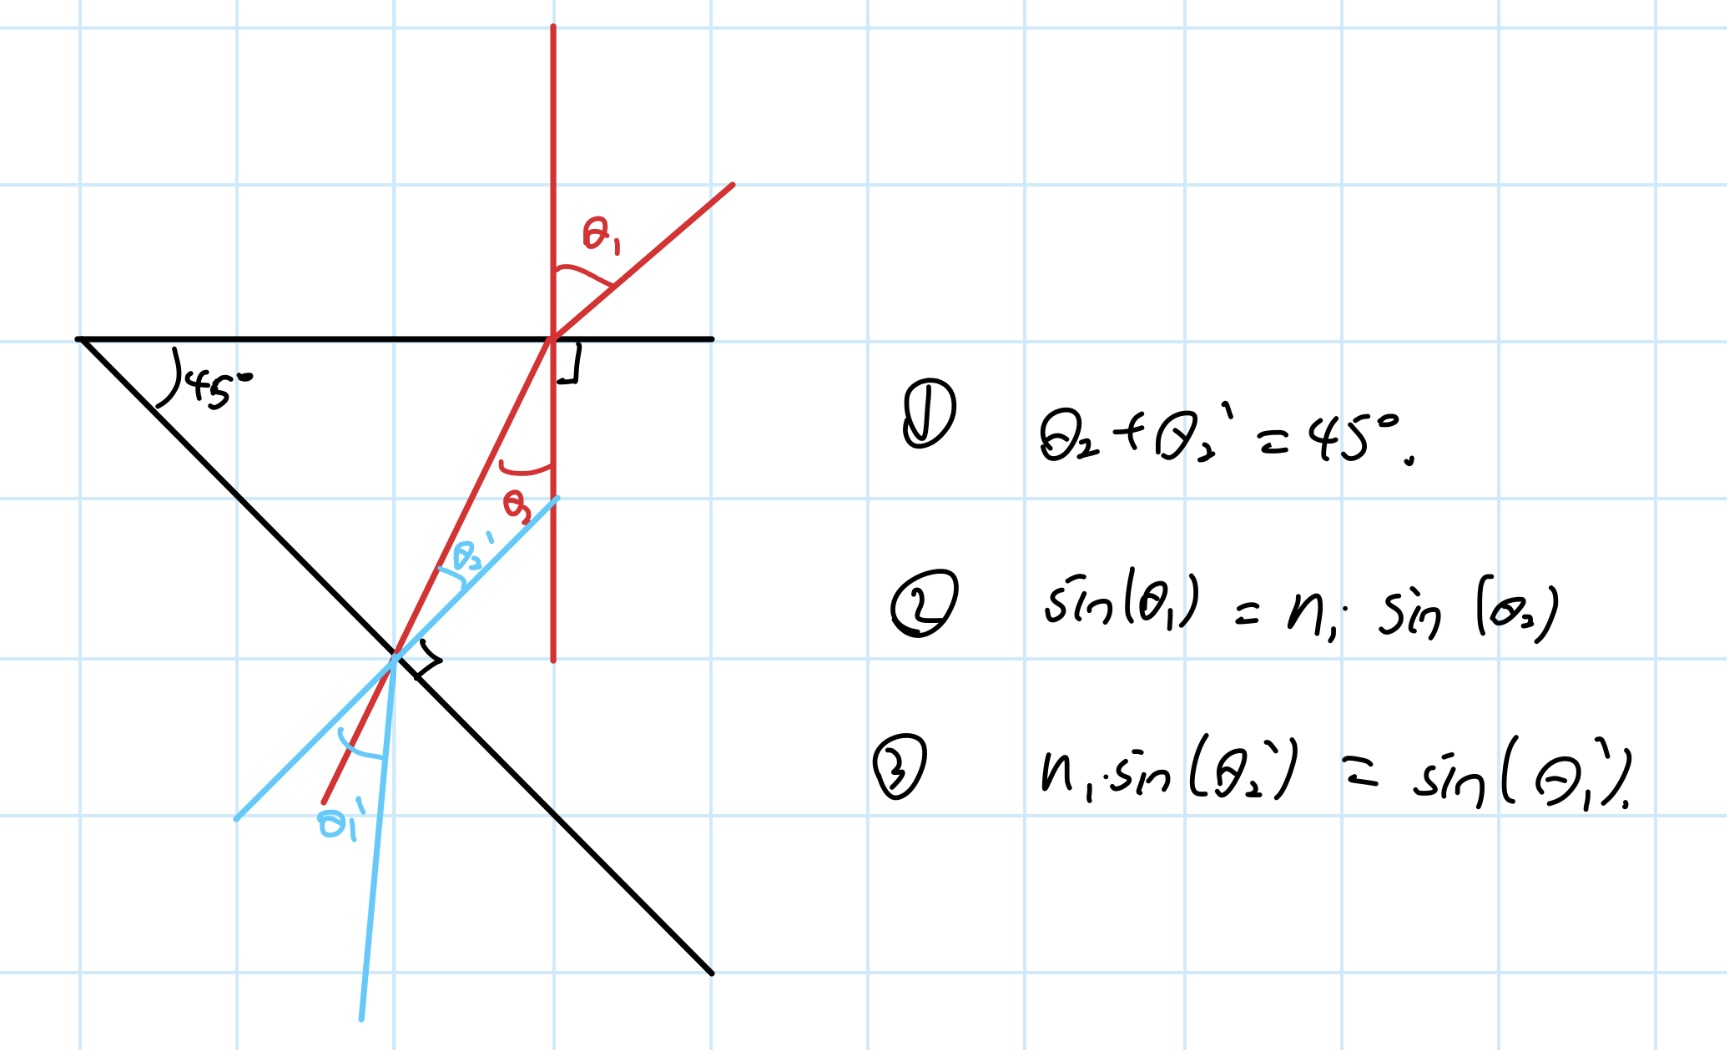
\includegraphics[width=120mm]{prism_rel.jpg}
    \caption{Triangular Prism's Angle Relation}
    \label{fig:prism_rel}
\end{figure}
\end{document}